\section{Results and Discussion}
\label{Sec:Res}

In this section, the proposed method using dataset a, b, c are compared to the recent non-deep-learning algorithms, such as Minh-CNN\cite{IEEEexample:mnih2013machine}, Satio-multi~\cite{IEEEexample:saito2016multiple} and Context~\cite{IEEEexample:audebert2017deep}.
%
Furthermore, it is also compared with some recent deep-learning based approaches, including FCN~\cite{IEEEexample:Long_2015_CVPR}, SegNet~\cite{IEEEexample:badrinarayanan2017segnet}, Deeplab~\cite{IEEEexample:chen2016deeplab} and U-Net~\cite{IEEEexample:ronneberger2015u}.\cxj{What else?}
Moreover for HF-FCN itself, we expect to investigate the effects of extracted information from different layers on the final prediction.
Thus, some variants which combine different up-sampling feature maps from Level 2 are proposed with details shown in Fig.~\ref{fig:Variants}.
In Fig.~\ref{fig:Variants}, we also compare our variants with the FCN to illustrate the differences between these two types of variants.
In addition, in order to find a better backbone network, we try the VGG16 Net and ResNet. The details are shown below.
\cxj{What about to change the backbone network?}

\begin{figure}[t]
\begin{center}
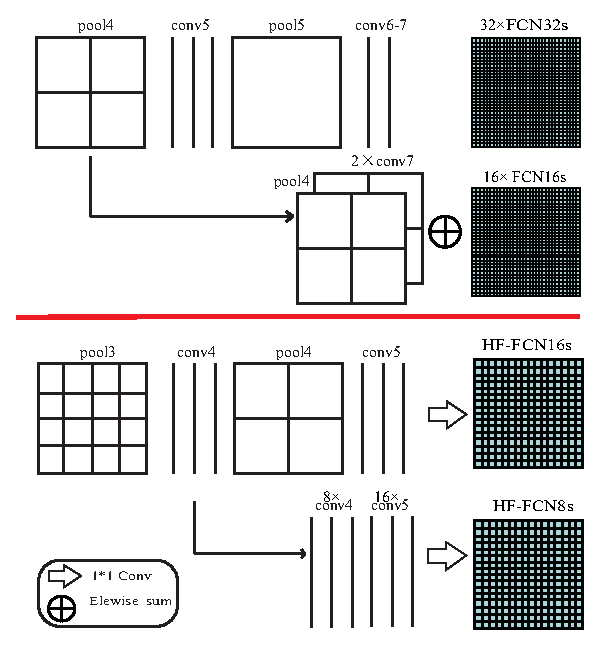
\includegraphics[width=7.8cm]{Figures/vairants.eps}
\caption{HF-FCN variants. The feature maps generated from final group are fused into a coarse result, which is HF-FCN16s. The variant called HF-FCN8s concatenates the feature maps from the last 2 groups with the same fusion operation, and so on.}
\label{fig:Variants}
\end{center}
\end{figure}

\subsection{Massachusetts dataset}
On the Massachusetts dataset, our method is compared to both the non-deep-learning algorithms and deep-learning based approaches. Table~\ref{table:Mass-results}\cxj{4} present the quantitative analysis. A standard and relaxed precision and recall are amply to make a comparison.
From the result, our method shows obvious superiority in terms of speed and precision. When comparing with Satio\-multi\-MA\&CIS, the standard and relaxed recall of our method are $5.5\%$ and $1.3\%$ higher than it. Meanwhile, the time cost is reduced from 67.84s to 1.07s and the speed is promoted about 63 times.
These significant improvements demonstrate that HF-FCN achieves best performance in effectiveness and efficiency.

Extensive comparisons are made between HF-FCN and other mainstream methods in semantic segmentation domain. The quantitative and visual results are shown in Table~\ref{table:Mass-results} and Fig.~\ref{fig:Mass-visi-result}, respectively. On the charts, we can see that our method better performance in speed and precision. And the details and integrity of the building are well preserved by our method.
\begin{table}
\centering
\caption {Correctness at breakeven of HF-FCN v.s. \cite{IEEEexample:mnih2013machine}\cite{IEEEexample:saito2016multiple}\cite{IEEEexample:alshehhi2017simultaneous} on Massachusetts test set. Cost time is computed in the same computer with a single NVIDIA Titan 12GB GPU}
\label{table:Mass-results}
\begin{tabular}{cccc}
\hline
&Recall ($\rho$ = 3)&Recall ($\rho$ = 0)&Time (s)\\
\hline
Mnih-CNN \cite{IEEEexample:mnih2013machine}&0.9271&0.7661&8.70\\
Mnih-CNN+CRF\cite{IEEEexample:mnih2013machine} &0.9282&0.7638&26.60\\
Satio-multi-MA \cite{IEEEexample:saito2016multiple}&0.9503&0.7873&67.72\\
Satio-multi-MA\&CIS \cite{IEEEexample:saito2016multiple}&0.9509&0.7872&67.84\\
Alshehhi-GAP+seg \cite{IEEEexample:alshehhi2017simultaneous}&0.955&{--}&{--} \\ \hline
FCN\_4s\cite{IEEEexample:Long_2015_CVPR}&0.839&0.6147&4.20\\
SegNet\cite{IEEEexample:badrinarayanan2017segnet}&0.7710&0.5675&2.39\\
U-Net\cite{IEEEexample:ronneberger2015u}& 0.9638& 0.8357& 3.165\\
DeepLab\_V2\cite{IEEEexample:chen2016deeplab}&0.9620&0.7575&1.89\\ \hline
HF-FCN(VGG16 Net)&0.9643&0.8424&1.07\\
HF-FCN(ResNet)&0.9588&0.8175&2.42\\
HF-FCN16s &0.9330&0.7233&0.85\\
HF-FCN8s &0.9643&0.8171&0.93\\
HF-FCN4s &0.9632&0.8394&0.99\\
\hline
\end{tabular}
\end{table}

To explore the effects of the feature maps generated from each conv layer on the final result, variants of HF-FCN which are counterpart of FCN are designed.
Unlike FCN, a fusion operation rather than summation are leveraged to build our HF-FCN 16s, 8s, 4s. Fig.~\ref{fig:Variants} shows the constrast diagram.
The performance of these variants are shown in Fig.~\ref{fig:Mass-variants-PR}, Fig.~\ref{fig:Mass-variants-visi} and Table~\ref{table:Mass-results}\cxj{Figure 8, Figure 9 and Table \Rmnum{5}}.
From the disgrams, we get the following conclusions. First, the prediction result obtained from the last layer gets a coarse result, which loses much of location information that are mainly encoded in the shallow feature maps. Second, the largest gap presented between HF-FCN16s and HF-FCN8s about 9{\%} in recall rates, it may suggest that the most information supplement to the HF-FCN is got in middle layers. Third, the PR curves of HF-FCN4s and HF-FCN almost coincide. It illustrates the low-level information has little effect on the prediction results. Forth, with the addition of the shallow feature map, the network is more distinct for the segmentation of tiny buildings, which solves the problem of easy adhesion to adjacent buildings. Since, all the conv layers contained useful hierarchical information that is critical to the final prediction.


In the end, we want to prove that our fusion operations learn the connections between features. Connection weights are shown in Fig.~\ref{fig:Mass-weights}. The weights are not the same, which means that fusion operation have effect on feature combination. From the Fig.~\ref{fig:Mass-weights} (f), we can arrive at the conclusion that the different layers have virous effect on the final result. For example, the U1\_1 has little effect on the prediction while the U3\_2 and U4\_3 have bigger role on the final prediction. It also in accordance with our experimental results that middle layers provide more information.
\cxj{Weight for what? to fuse feature map? The distribution does not make too much sense. } 

\begin{figure}
\centering
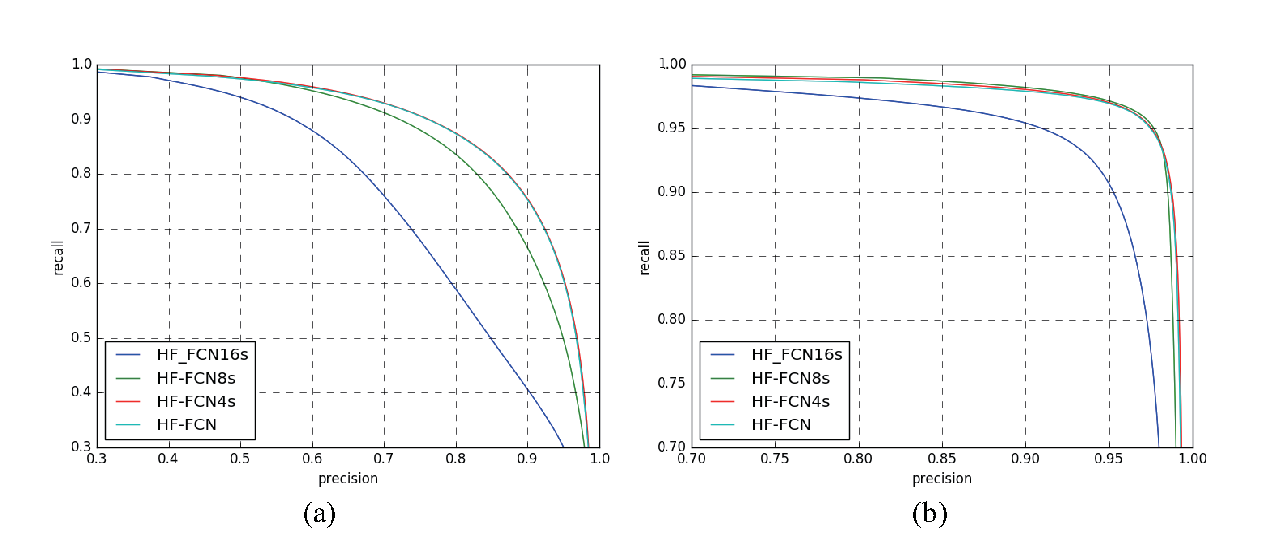
\includegraphics[width=8.7cm]{Figures/HF-FCN-variant-PR.eps}
\caption{The relaxed precision-recall curves from HF-FCN variants with two slack paramters. The biggest gap occurs between HF-FCN16s and HF-FCN8s, which indicates the most additional information coming from middle layers.}
\label{fig:Mass-variants-PR}
\end{figure}

\begin{figure}
\centering
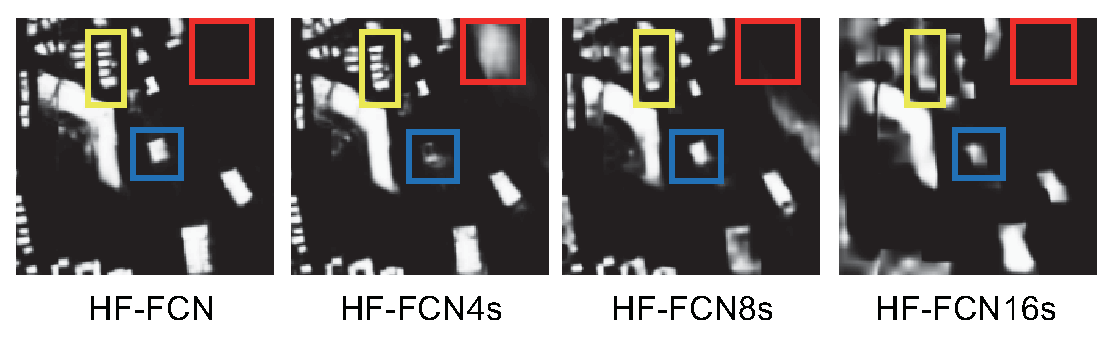
\includegraphics[width=8.7cm]{Figures/HF-FCN_variants_result.eps}
\caption{Prediction results of HF-FCN, HF-FCN4s, HF-FCN8s and HF-FCN16s. The yellow box shows the continuous refinement of the tiny buildings. The red and blue boxes show the mutual promotion and contradiction between different layers.}
\label{fig:Mass-variants-visi}
\end{figure}

\begin{figure*}
\centering
\includegraphics[width=17cm,height = 7cm]{Figures/mass_visi_result.eps}
\caption{(a) input images. (b) Results of Mnih-CNN+CRF. (c) Results of Satio\-multi\-MA\&CIS. (d) Results of FCN4s . (e) Results of SegNet. (f) Results of DeepLab\_V2. (g) Results of U-Net. (h) Our results. TP are shown in green, FP are shown in blue and FN are in red.}
\label{fig:Mass-visi-result}
\end{figure*}

\begin{figure}
\centering
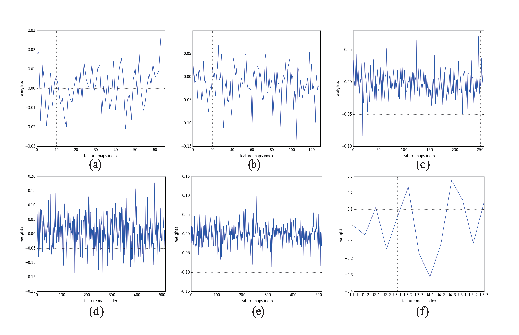
\includegraphics[width=9cm]{Figures/weights.eps}
\caption{(a) is weights learned by F1\_1, (b) is weights learned by F2\_1, (c) is weights learned by F3\_1, (d) is weights learned by F4\_1, (e) is weights learned by F5\_1, (f) is weights learned by Level 2.}
\label{fig:Mass-weights}
\end{figure}

\subsection{Vaihingen dataset}
On Vaihingen dataset, three experiments are undertaken to explore the effects of different inputs, diverse variants and various methods. We utilize three kinds of combinations of image channels as inputs. The inputs of the 3 channels are IR, R, G and adding the nDSM as the forth channel. Based on it, DSM is added and made up 5-channel input. We use three standards to make a more comprehensive evaluation. The evaluation results are shown in Table~\ref{table:vaihigen-3-4-5in-comp}, which illustrates that 3-channel input performed better than the other. The Rec and Pre in Table~\ref{table:vaihigen-3-4-5in-comp} means the recall and precision of prediction results. And F1 indicates the F1\_score of results. The number in bold shows the best results in validation and test set. Corresponding visual results are shown in Fig. ~\ref{fig:Vaihingen-3-4-5in}.

\cxj{Do you compare with others?}


\begin{table*}[htbp]
\caption {Performance comparison of the results of different inputs on Vaihigen data set. \cxj{What are the numbers in the Img column?}}
\label{table:vaihigen-3-4-5in-comp}
\centering
\begin{tabular}{p{1.1cm}<{\centering}|p{1.1cm}<{\centering}|p{1.1cm}<{\centering}|p{1.1cm}<{\centering}|p{1.1cm}<{\centering}|p{1.1cm}<{\centering}|p{1.1cm}<{\centering}|p{1.1cm}<{\centering}|p{1.1cm}<{\centering}|p{1.1cm}<{\centering}|p{1.1cm}<{\centering}}
\hline
&\multirow{2}{*}{Img}&\multicolumn{3}{c}{3\_in: IR, R, G} &\multicolumn{3}{|c|}{4\_in: IR, R, G, nDSM}&\multicolumn{3}{c}{5\_in: IR, R, G, DSM, nDSM}\\
\cline{3-11}
&& Pre &Rec & F1 &Pre &Rec &F1&Pre &Rec &F1\\
\hline
\multirow{3}{*}{Val}&11&0.911&0.906&0.909&0.936&0.900&0.917&0.890&0.900&0.900\\
&28&0.94&0.875&0.906&0.96&0.792&0.868&0.952&0.823&0.883\\
&34&0.965&0.899&0.930&0.987&0.902&0.942&0.972&0.918&0.944\\
&Ave&0.939&0.894&$\bm{0.915}$&0.961&0.865&0.909&0.939&0.880&0.907\\
\hline
\multirow{2}{*}{Test}&15&0.918&0.930&0.924&0.883&0.917&0.9&0.833&0.931&0.88\\
&30&0.921&0.929&0.926&0.931&0.827&0.876&0.875&0.877&0.876\\
&Ave&0.919&0.930&$\bm{0.925}$&0.907&0.872&0.888&0.858&0.900&0.878\\
\hline
\end{tabular}
\end{table*}

We compare with some other methods which use the same dataset. The detail comparison results are shown in Fig.~\ref{fig:Vaihingen-compared-others}. From a visual perspective, our method gets a much more refined roof region, both on continuity of labels and integrity of structural.

The results of diverse variants are shown in Fig.~\ref{fig:Vaihingen-variants}. The HF-FCN\_1 in Fig.~\ref{fig:Vaihingen-variants} indicates that the last conv layer in Level 2 does not use the previous trained model to initialize. And HF-FCN means that the whole layers use the pre-trained model to initialize. From the curves, the performance of HF-FCN exceeds the variants and gets a excellent result. Additionally, using the pre-trained weights of Level 2 has a significance in the final results.

\begin{figure}
\centering
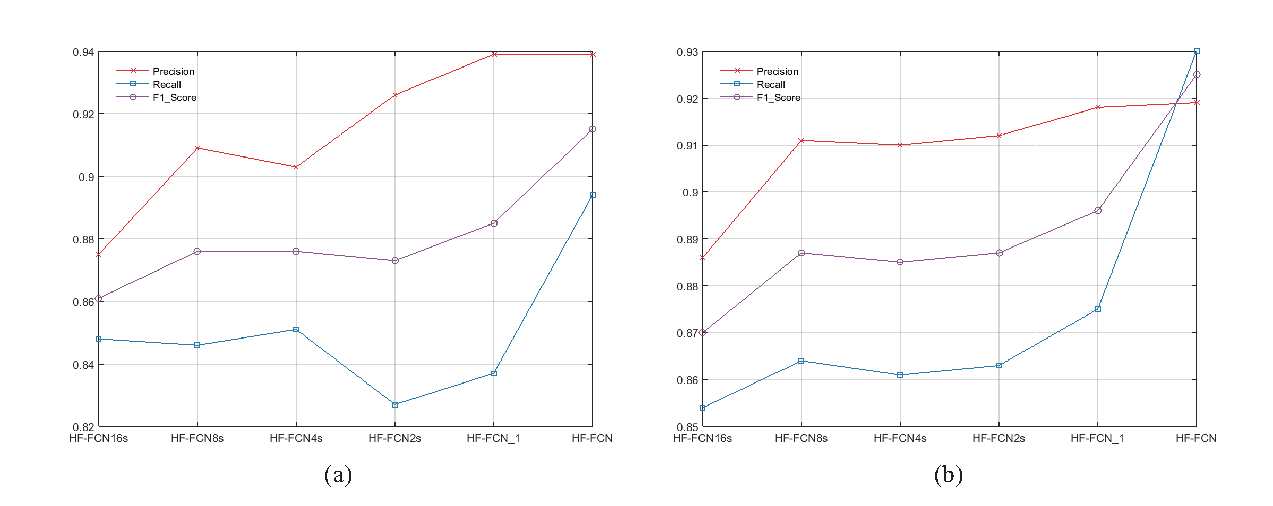
\includegraphics[width=8.7cm]{Figures/vaihingen_variants.eps}
\caption{Results of HF-FCN variants on Vaihingen dataset. (a) (b) shows the precision, recall and F1\_score of validation set and test set of Vaihingen dataset respectively.\cxj{Bigger font}}
\label{fig:Vaihingen-variants}
\end{figure}

\begin{figure}
\centering
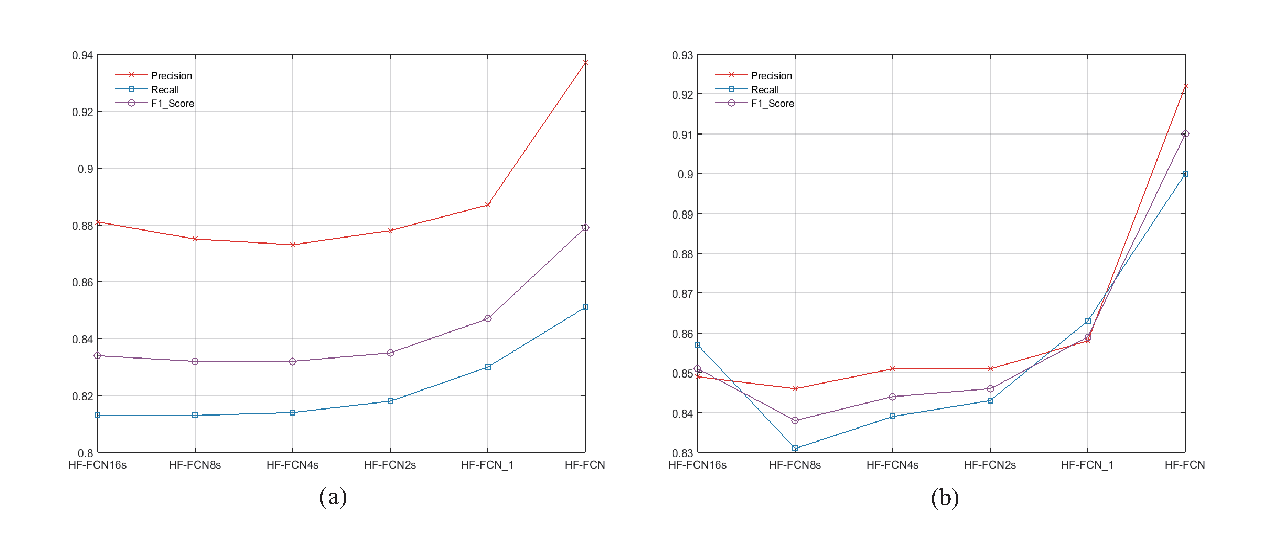
\includegraphics[width=8.7cm]{Figures/Potsdam_variants.eps}
\caption{Results of HF-FCN variants on Potsdam dataset. (a) (b) shows the precision, recall and F1\_score of validation set and test set of Potsdam dataset respectively.}
\label{fig:Potsdam-variants}
\end{figure}

\begin{figure}
\centering
\includegraphics[width=8.7cm]{Figures/Vaihingen3_4_5in.eps}
\caption{Prediction results on Vaihingen dataset. (a) (b) (c) shows results of the 3-channel input, 4-channel input and 5-channel input of Vaihingen dataset respectively. Here, TP are shown in green, FP are shown in blue and FN are in red.}
\label{fig:Vaihingen-3-4-5in}
\end{figure}

\begin{figure}
\centering
\includegraphics[width=8.7cm]{Figures/Vaihingen_compared_results.eps}
\caption{Results of different methods. (a) is input image, (b)(d)(g) are results of \cite{IEEEexample:audebert2017deep}, (c) is result of \cite{IEEEexample:marmanis2016semantic}, (f) is result of \cite{IEEEexample:unknown}, (g) is our result. The blue and yellow frames show some details between these methods.}
\label{fig:Vaihingen-compared-others}
\end{figure}


\subsection{Potsdam dataset}
 The same experiments are implemented on Potsdam dataset. First, We utilize DSM and IR information as extra inputs based on the RGB input. The specific quantitative evaluation and intuitive visual prediction results are shown in Table~\ref{table:Potsdam-3-4-5in-comp} and Fig.~\ref{fig:Potsdam-3-4-5in-visi}. In the validation process, the 4-channel input gets better overall performance. Meanwhile, the 5-channel input seems perform better in the course of testing. From the visual results, the 5-channel input network gets lower error detection rate which is shown on the image with small blue areas. And from the 3-channel input to 5-channel input, the F1 score increases from 0.879 to 0.891 on the validation set and increases 0.031 on the test set. It indicate that the other information of geographical feature have a certain effect on the final result.
 
 We compare HF-FCN with other methods using the Potsdam dataset. Some qualitative results are shown in Fig.~\ref{fig:Potsdam-compared-others}. 
 From the figure, we can easily see that HF-FCN got more remarkable segmentation results. And edges and structure of buildings are preserved better.
 
 As done on Vaihingen dataset, contrast experiments of HF-FCN variants are implemented. The performance curve of HF-FCN variants are shown in Fig.~\ref{fig:Potsdam-variants}.
 The HF-FCN\_1 in Fig.~\ref{fig:Potsdam-variants} indicates that the last conv layer in Level 2 does not use the previous trained model to initialize. And HF-FCN means that the whole layers use the pre-trained model to initialize. Initialization of parameters has a greater promotion on the final results.

\begin{table*}[htbp]
    \caption {Performance comparison of the results of different inputs on Potsdam data set}
    \label{table:Potsdam-3-4-5in-comp}
    \begin{center}
    \begin{tabular}{p{1.1cm}<{\centering}|p{1.1cm}<{\centering}|p{1.1cm}<{\centering}|p{1.1cm}<{\centering}|p{1.1cm}<{\centering}|p{1.1cm}<{\centering}|p{1.1cm}<{\centering}|p{1.1cm}<{\centering}|p{1.1cm}<{\centering}|p{1.1cm}<{\centering}|p{1.1cm}<{\centering}}
     \hline
    &\multirow{2}{*}{Img}&\multicolumn{3}{c}{3\_in:RGB} &\multicolumn{3}{|c|}{4\_in:RGB,IR}&\multicolumn{3}{c}{5\_in:RGB,IR,nDSM}\\
     \cline{3-11}
    && Pre &Rec & F1 &Pre &Rec &F1&Pre &Rec &F1\\
    \hline\hline
    \multirow{4}{*}{Val}&2\_11&0.917&0.950&0.933&0.917&0.978&0.946&0.934&0.976&0.954\\
    &4\_10&0.937&0.945&0.941&0.926&0.943&0.936&0.947&0.946&0.946\\
    &5\_11&0.930&0.972&0.950&0.959&0.975&0.966&0.956&0.977&0.967\\
    &7\_10&0.964&0.536&0.689&0.950&0.590&0.728&0.939&0.554&0.697\\
    \cline{2-11}
    &{Average}&0.937&0.851&0.879&0.937&$\bm{0.872}$&$\bm{0.894}$&$\bm{0.944}$&0.864&0.891\\
    \hline\hline
    \multirow{3}{*}{Test}&2\_12&0.897&0.868&0.882&0.920&0.959&0.939&0.944&0.965&0.955\\
    &6\_7&0.894&0.902&0.898&0.915&0.909&0.912&0.901&0.918&0.909\\
    &7\_8&0.975&0.929&0.951&0.977&0.950&0.957&0.976&0.946&0.960\\
    \cline{2-11}
    &{Average}&0.922&0.900&0.910&0.937&0.935&0.936&$\bm{0.940}$&$\bm{0.943}$&$\bm{0.941}$\\
    \hline\hline
   \end{tabular}
   \end{center}
   \end{table*}

\begin{figure}
\centering
\includegraphics[width=8.7cm]{Figures/Potsdam3_4_5in.eps}
\caption{Prediction results on potsdam dataset. (a) (b) (c) shows results of the 3-channel input, 4-channel input and 5-channel input of Vaihingen dataset respectively. Here, TP are shown in green, FP are shown in blue and FN are in red.}
\label{fig:Potsdam-3-4-5in-visi}
\end{figure}

\begin{figure}
\centering
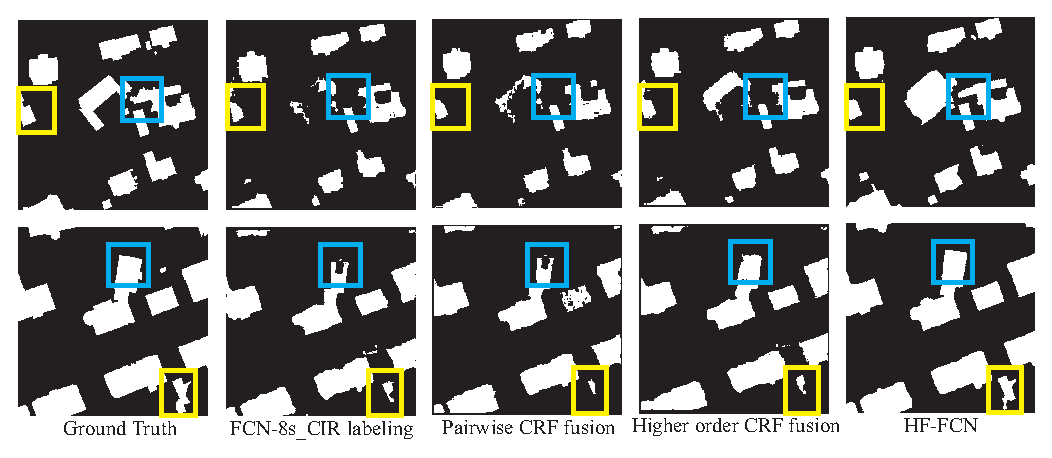
\includegraphics[width=8.7cm]{Figures/Potsdam_compared_results.eps}
\caption{Results of different methods. The second column is the results of using only the FCN with CIR. Pairwise CRF fusion shows the result of fusing FCN-8s\_CIR with LiDAR data in a pairwise CRF. Higher-order CRF are used to generate the results shown in third column. Our results are shown in last colunm.}
\label{fig:Potsdam-compared-others}
\end{figure}
